\section{电动势产生的机理}

    \subsection{界面电势差}

    在水合作用下,一部分金属离子可以离开金属进入水层之中。这会导致金属带负电,溶液带正电,如图\ref{fig:surface_E}所示。

    \begin{figure}[h]
        \centering
        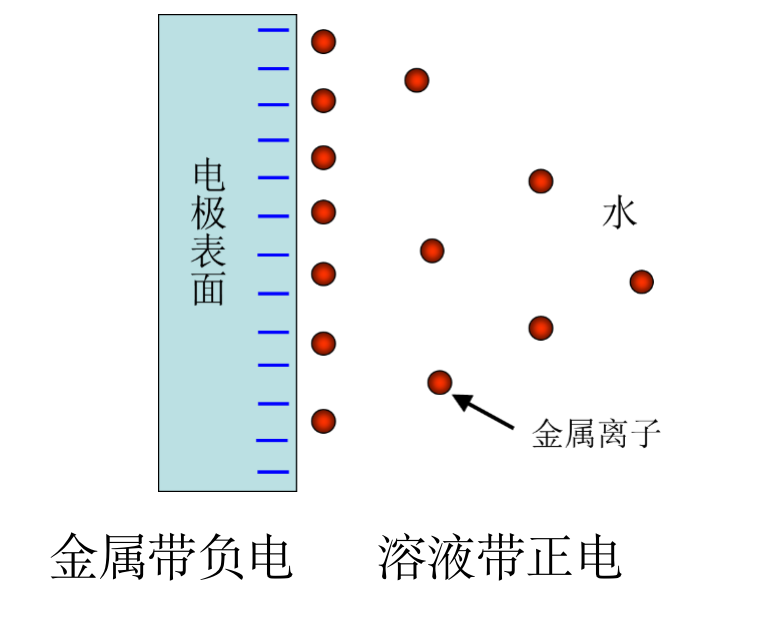
\includegraphics[width=0.6\textwidth]{surface_E.png}
        \caption{界面电势差的形成}
        \label{fig:surface_E}
    \end{figure}
    
    \subsubsection{紧密层}
    在金属与溶液的界面上,由于正、负离子静电吸引和热运动两种效应的结果,溶液中的金属离子只有一部分紧密地排在固体表面附近,相距约一、二个离子厚度。
    \subsubsection{扩散层}
    另一部分离子按一定的浓度梯度扩散到本体溶液中。

    \subsubsection{双电层}

    电极表面电荷层和溶液多余反离子构成\textbf{双电层}(见图\ref{fig:surface_E_layers})。金属表面和溶液本体之间的电势差即为界面电势差。

    
    \begin{figure}[h]
        \centering
        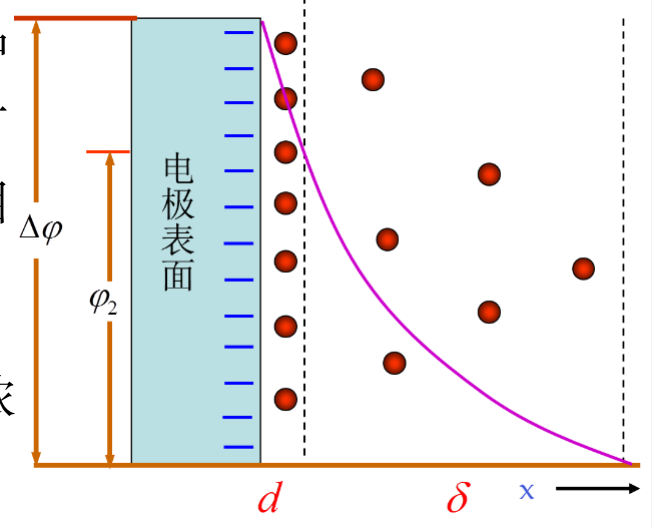
\includegraphics[width=0.6\textwidth]{surface_E_layers.png}
        \caption{紧密层-扩散层}
        \label{fig:surface_E_layers}
    \end{figure}


    

    \subsection{接触电势}

    电子逸出功,电子从金属表面逸出时,为了克服表面势垒所做的功。相互接触时,逸出功的大小不一致,导致表面间存在接触电势。


    \subsection{液体接界电势}

    在含有不同溶液的形成的界面上,或同一种溶液不同浓度所形成的的界面上,由于阴阳离子迁移的速度不一致,会导致界面形成微小的电动势。这一电动势被称为液接电势(图\ref{fig:ljp})。

    \begin{figure}[h]
        \centering
        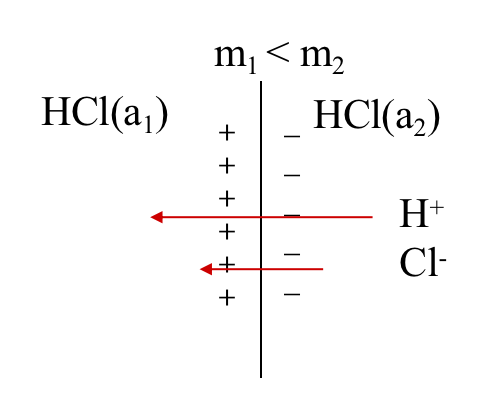
\includegraphics[width=0.6\textwidth]{ljp.png}
        \caption{液接电势的形成}
        \label{fig:ljp}
    \end{figure}

    \subsubsection{盐桥的作用}

    液接电势对电动势产生干扰,可以用\textbf{盐桥}(图\ref{fig:salt_bridge})来抵消液接电势。


    \begin{figure}[h]
        \centering
        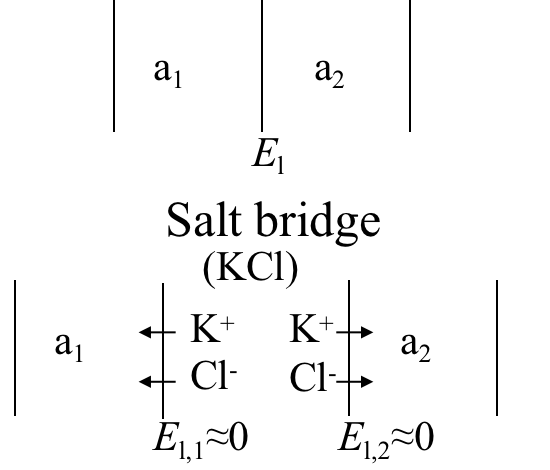
\includegraphics[width=0.6\textwidth]{salt_bridge.png}
        \caption{盐桥的作用}
        \label{fig:salt_bridge}
    \end{figure}

    \section{电动势的计算}

    \subsection{直接加和}

    将电池中各种界面的电势差加起来,为电动势。

    \subsection{通过Nernst方程计算}

    \begin{reaction*}
        Pt | H2(p1) | HCl(a) | Cl2(p2) | Pt
    \end{reaction*}

    \begin{equation*}
        \Delta_r G_m = \Delta_r G_m ^\ominus + RT\ln \prod _{B} a_B^{\nu_B}
    \end{equation*}

    根据$\Delta_r G_m = -zFE$

    \begin{equation*}
        E = E^\ominus - \frac{RT}{zF} \ln \prod _{B} a_B^{\nu_B}
    \end{equation*}

    这里的$z$取多少并不会影响最后电动势的大小,整体变化$z$的话,系数会在对数部分得到还原。

    \begin{reaction*}
        Pt | H2( $p$ ) | H2SO4 | O2(p) | Pt
    \end{reaction*}


    \begin{reactions*}
        H2 - 2 e- &-> 2 H+ \\
        1/2 O2 + 2 e- + 2 H+ &-> H2O
    \end{reactions*}

    \subsection{电极电势}

    认为氢标准电极的电势为0,其他电极的电势是相对的电势。电极电势为负数时表示容易进行氧化反应,电极电势为正数时,容易发生还原反应。

    $\phi^{\ominus}$ 标准电极电势,在标准状态下的材料制备时的$\phi$。$\phi$是与氢标准电极形成原电池下的$E$。$\phi$的计算与$E$相同。

    \begin{equation*}
        \Delta_r G_m = -zF\phi
    \end{equation*}

    \begin{equation*}
        \Delta_r G_m ^\ominus = -zF\phi ^\ominus
    \end{equation*}

    \begin{reaction*}
        Zn^{2+} (a1) + 2 e- -> Zn
    \end{reaction*}

    \begin{equation*}
        \phi_{ \left( \ch{Zn^{2+} | Zn} \right) } = \phi^\ominus - \frac{RT}{zF} \ln \frac{1}{a1}
    \end{equation*}